\documentclass[12pt]{article}
\usepackage[utf8x]{inputenc}
\usepackage[usenames,dvipsnames,svgnames]{xcolor}
\usepackage{amsmath}
\usepackage{graphicx}
\usepackage{float}
\usepackage{dsfont}
\usepackage{amsfonts}
\usepackage[T1]{fontenc}
\usepackage[colorinlistoftodos]{todonotes}
\usepackage[margin=2.5cm,a4paper]{geometry}
\usepackage{listings}
\usepackage{minted}
\usepackage{multicol}
\usepackage{fancyhdr}
\usepackage{cite}
\usepackage{cleveref}
\usepackage{siunitx}
\setlength{\parindent}{0pt}
\newcommand{\deriv}{\mathrm{d}}
\usepackage{color}  
\usepackage{hyperref}
\hypersetup{
    colorlinks=true, 
    linktoc=all,    
    linkcolor=black, 
    citecolor=black,
}
\lstset{
    language=R,
    basicstyle=\scriptsize\ttfamily,
    commentstyle=\ttfamily\color{red},
    numbers=left,
    numberstyle=\ttfamily\color{blue}\footnotesize,
    stepnumber=1,
    numbersep=5pt,
    backgroundcolor=\color{white},
    showspaces=false,
    showstringspaces=false,
    showtabs=false,
    frame=single,
    tabsize=2,
    captionpos=b,
    breaklines=true,
    breakatwhitespace=false,
    title=\lstname,
    escapeinside={},
    keywordstyle={},
    morekeywords={}
}

\pagestyle{fancy}
\fancyhf{}
\rhead{PH370 Computing}
\lhead{C3 - Weather Station Assignment}
\rfoot{-\thepage\centering-}

\begin{document}
\begin{titlepage}

\newgeometry{left=1.5in,right=1.5in,top=2.5in,bottom=2.5in}
\newcommand{\HRule}{\rule{\linewidth}{0.5mm}}

\begin{centering} 
 
%------------------------------------------------------------------------
%	HEADING SECTIONS
%------------------------------------------------------------------------


\includegraphics[scale=0.4]{Uni_of_Kent_Logo.png}\\[1cm]

%------------------------------------------------------------------------
%	TITLE SECTION
%------------------------------------------------------------------------

\HRule \\[0.4cm]
\textsc{\large Astronomy, Space Science and Astrophysics}\\[0.4cm]
{\huge \bfseries Weather Station Assignment}\\[0.4cm]
\HRule \\[1.0cm]

%------------------------------------------------------------------------
%	DATE SECTION
%------------------------------------------------------------------------

\textsc{\Large Stage 1 - PH370 Computing}\\[0.5cm] 
{\large Monday 5th March 2018}\\[1.0cm]

%------------------------------------------------------------------------
%	AUTHOR SECTION
%------------------------------------------------------------------------

\begin{minipage}{0.625\textwidth}
\centering

\emph{\large Report Author:} \large Lukasz R Tomaszewski \\ [0.2cm]
\end{minipage}\\[2cm]

\vfill
\end{centering} 
\end{titlepage}

%------------------------------------------------------------------------
%------------------------------------------------------------------------
%	CONTENTS  
%------------------------------------------------------------------------
%------------------------------------------------------------------------

\newpage
\begin{titlepage}
\begin{tableofcontents}

\end{tableofcontents}
\end{titlepage}

%-----------------------------------------------------------------------
%-----------------------------------------------------------------------
%	INTRODUCTION   
%-----------------------------------------------------------------------
%-----------------------------------------------------------------------

\section{Introduction}

Within this assignment, a collection of weather station data over three years has containing fourteen variables of data e.g. wind speed, temperature, wind direction, etc. With this mass collection of data there are many ideas for a investigations to find a correlation between 2 or more of the variables of data. This allows connections to be made between set data and thus help predict future occurrences when the pattern of the correlation of data connects. The purpose of this assignment as stated above is to find a correlation between two or more of the variables of data, the chosen investigation which is stated in this report is; \\

"Whether an correlation exists between wind speed and temperature. Whether the coldest/ hottest temperatures are associated with fast/ slow wind speeds". The following idea for investigation comes from \cite{Weather_Station}, this was chosen as the hypothesis of a strong connection between temperature and wind speed must be true due to the scientific fact of hot temperatures makes molecules increase in size and gain velocity and thus cold temperatures make molecules decrease in size and lose velocity.

%-----------------------------------------------------------------------
%-----------------------------------------------------------------------
%	METHOD
%-----------------------------------------------------------------------
%-----------------------------------------------------------------------

\section{Method}

The programming software Python, was used to analyze the data across three .csv spreadsheet files, and then plot the data on graphs that will allow any correlations or connection between the data to be found. In section \ref{Python Script}, is the code used to analyze the data and plot the data on scatter graphs that was collected from the three .csv files. The outputted graphs are found in section \ref{Main Results}. \\

The fourth graph in section \ref{Main Results} shows a density graph representing all three years worth of data instead of a single year, this allows for a connection to be made over a long period of time proving its a common occurrence. Using the concentrate command line in python, the multiple sources of data can be complied under two domains and be plotted using the hexbins command that allows the data to be plotted in a density graph instead of a scatter graph. \\

All three years worth of data is plotted on their own individual graphs and the density graph to be plotted again separately to allow for a separate analysis. The graphs can now be analyzed for any correlations and relationships of reoccurring occurrences.

%-----------------------------------------------------------------------
%-----------------------------------------------------------------------
%	RESEARCH
%-----------------------------------------------------------------------
%-----------------------------------------------------------------------

\section{Research}
\label{Research Section}

Understanding how temperature directly affects wind speed is key to prove whether the chosen hypothesis is true or false, using the website \href{https://www.metoffice.gov.uk/learning/weather-for-kids/understanding-weather}{Understanding Weather} detail founds in \cite{Weather_Research}, this allows for an accurate analysis of data if there are any errors that occur within the data. The research states that there is a direct relationship with temperature and air pressure with air pressure being a main factor of wind speed, thus proving a scientific connection between the chosen whether elements data and that higher wind speeds result in lower temperature. \\

%-----------------------------------------------------------------------
%-----------------------------------------------------------------------
%	ANALYSIS
%-----------------------------------------------------------------------
%-----------------------------------------------------------------------

\pagebreak
\section{Analysis}

Starting with comparing temperature and wind speed in the year 2015 shown in figure \ref{Temperature Vs Wind Speed graph for 2015.}, a correlation already exists between both variables of data that the lower wind speed is a directly result of low temperature. Unfortunately the weather station that collects the data variables was off-line for a few months during the year 2015 thus the data collected from this year does not accurately prove that the correlation is there. \\

During the year 2016, the weather station collected data throughout the whole year unlike the data collected in 2015, the data for 2016 is shown in figure \ref{Temperature Vs Wind Speed graph for 2016.} but does not show a accurate correlation between low temperature and low wind speed. This disproves the hypothesis but the graph does show a strong cluster between 0-20 degrees and wind speeds under 20 kph (kilometers per hour), even though this does not specifically relate to the hypothesis, it is a key factor to note. \\

Much like 2015, there is only a brief amount of data from the year 2017 shown in figure \ref{Temperature Vs Wind Speed graph for 2017.} thus this data cannot fully support the hypothesis but does again show the same key factor shown in the 2016 data show in figure \ref{Temperature Vs Wind Speed graph for 2016.} the same cluster between 0-20 degrees and wind speeds under 20 kph (kilometers per hour). As only there is only one whole years worth of data that represents seasonal change of the planet Earth rotation around the Sun causing different temperature and wind speeds during the different seasons of the year then the data is not enough to support the hypothesis. \\

The hypothesis is currently not accurately supported thus another graph must be made to concentrate all three years worth of data even though two of the three years have incomplete data, the data provided shows strong clusters. Analyzing the data in found in figure \ref{Temperature Vs Wind Speed graph for 2015/ 16/ 17.} is the priority graph to observe and accurate observations, within this section, correlations have been made but only to a specific year and a short time frame, figure \ref{Temperature Vs Wind Speed graph for 2015/ 16/ 17.} shows not only one year but all three years thus showing a strong accurate correlation over a long period of time. It shows that the lower the temperature (higher humidity) there are lower wind speeds compared to the higher temperature (lower humidity) and high wind speeds. \\

In conclusion of the analysis of the weather station in relation of the original hypothesis \cite{Weather_Station}; \\

"Whether an correlation exists between wind speed and temperature. Whether the coldest/ hottest temperatures are associated with fast/ slow wind speeds". \\

As the data from 2015 and 2017 are incomplete, there is no accurate answer to the selected hypothesis but using the data that was collected then, there is a strong cluster showing a correlation within the margin of low wind speeds under 20 kph (kilometers per hour) within the temperature range of 0-20 degrees, as stated in section \ref{Research Section} there is a connection between temperature affecting air pressure which directly relates to the velocity of the wind. Using the research, the hypothesis is proven to be correct but with the data collected by the weather station at the University of Kent due to the incomplete data sets, it cannot be proven from said data. 

%-----------------------------------------------------------------------
%-----------------------------------------------------------------------
%	MAIN RESULTS
%-----------------------------------------------------------------------
%-----------------------------------------------------------------------

\pagebreak
\section{Main Results}
\label{Main Results}

\begin{figure}[H]
\centering
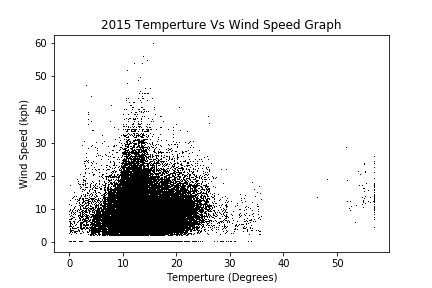
\includegraphics[scale=1.0]{Graphs/2015_Temperture_Vs_Wind_Speed.png}
\caption{Temperature Vs wind speed graph for 2015.}
\label{Temperature Vs Wind Speed graph for 2015.}
\end{figure}

\begin{figure}[H]
\centering
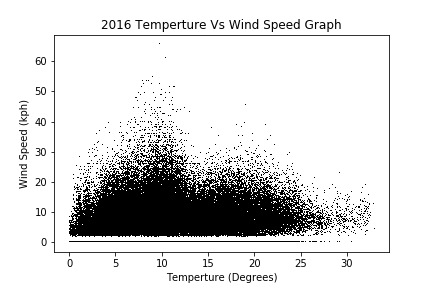
\includegraphics[scale=1.0]{Graphs/2016_Temperture_Vs_Wind_Speed.png}
\caption{Temperature Vs wind speed graph for 2016.}
\label{Temperature Vs Wind Speed graph for 2016.}
\end{figure}

\begin{figure}[H]
\centering
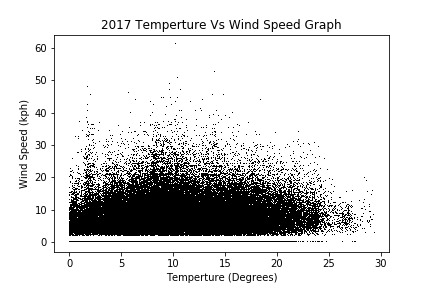
\includegraphics[scale=1.0]{Graphs/2017_Temperture_Vs_Wind_Speed.png}
\caption{Temperature Vs wind speed graph for 2017.}
\label{Temperature Vs Wind Speed graph for 2017.}
\end{figure}

\begin{figure}[H]
\centering
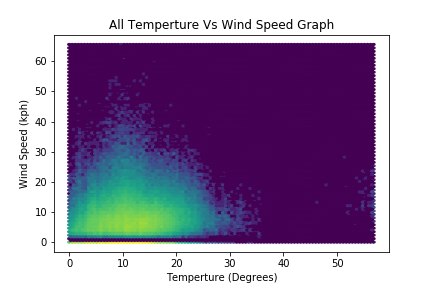
\includegraphics[scale=1.0]{Graphs/All_Temperture_Vs_Wins_Speed.png}
\caption{Temperature Vs wind speed graph for 2015/ 16/ 17.}
\label{Temperature Vs Wind Speed graph for 2015/ 16/ 17.}
\end{figure}

%-----------------------------------------------------------------------
%-----------------------------------------------------------------------
%	PYTHON SCRIPT
%-----------------------------------------------------------------------
%-----------------------------------------------------------------------

\pagebreak
\section{Python Script}
\label{Python Script}

\begin{minted}[bgcolor=AliceBlue]{python3}

import matplotlib.pylab as plt
import numpy as np
#Line 9 - 10 contain both packages that'll help develop the graphs.
#Matplotlib.pylab will help in the development of graphing the data.
#Numpy helps analyze the data and puts them in a dedicated order.

x15, y15 = np.genfromtxt('Weather_2015.csv',delimiter=',',
                         usecols=[1,7],unpack=True)
filter15 = np.logical_and(x15 >= 0, y15 >= -100)
print('Analysis of Weather 2015 Data Completed')
#Lines 15 - 18, the numpy package selected only column 1 and 7 which 
#are the columns containing the data for temperture and wind speed of
#the year 2015, this data is set as temperture being the x-axis and 
#wind speed being the y-axis. This data is then plotting on a graph.
#The filter command is to only highlight data that is above 0 and -100,
#this allows the a smaller ammount of data that is more accurate to the
#hypothesis, it is the data more relevant.
#The print command allows the user to know that the data for
#Weather2015.csv that it has been read and is ready to plot onto a graph.

x16, y16 = np.genfromtxt('Weather_2016.csv',delimiter=',',
                         usecols=[1,7],unpack=True)
filter16 = np.logical_and(x16 >= 0, y16 >= -100)
print('Analysis of Weather 2016 Data Completed')
#Lines 29 - 32, the numpy package selected only column 1 and 7 which 
#are the columns containing the data for temperture and wind speed of
#the year 2016, this data is set as temperture being the x-axis and 
#wind speed being the y-axis. This data is then plotting on a graph.
#The filter command is to only highlight data that is above 0 and -100,
#this allows the a smaller ammount of data that is more accurate to the
#hypothesis, it is the data more relevant.
#The print command allows the user to know that the data for
#Weather2016.csv that it has been read and is ready to plot onto a graph.

x17, y17 = np.genfromtxt('Weather_2017.csv',delimiter=',',
                         usecols=[1,7],unpack=True)
filter17 = np.logical_and(x17 >= 0, y17 >= -100)
print('Analysis of Weather 2017 Data Completed')
#Lines 43 - 46, the numpy package selected only column 1 and 7 which 
#are the columns containing the data for temperture and wind speed of
#the year 2017, this data is set as temperture being the x-axis and 
#wind speed being the y-axis. This data is then plotting on a graph.
#The filter command is to only highlight data that is above 0 and -100,
#this allows the a smaller ammount of data that is more accurate to the
#hypothesis, it is the data more relevant.
#The print command allows the user to know that the data for
#Weather2017.csv that it has been read and is ready to plot onto a graph.

x = np.concatenate((x15[filter15],x16[filter16],x17[filter17]))
y = np.concatenate((y15[filter15],y16[filter16],y17[filter17]))
#Much like the other group of code, line 57 & 58 allow the user to 
#only plot the filtered data onto a seperate graph which is located
#on line 99-105 and is the last graph plotted, this allows for a density 
#graph to be plotted and therefore an accurate comparsion across all 
#three years worth of data instead of a specfic year. Thus allowing 
#to find a strong correlation over a long period of time instead of a 
#short period of time.

plt.plot(x15[filter15],y15[filter15],'k,')
plt.xlabel('Temperture (Degrees)')
plt.ylabel('Wind Speed (kph)')
plt.title('2015 Temperture Vs Wind Speed Graph')
plt.savefig('2015 Temperture Vs Wind Speed.png')
#Lines 67-71 print a graph that plots the data collected from the
#Weather2015.csv file in line 15-18. This group of code plots the 
#data and labels the xy axis of the graph and gives the graph a title.
#Line 71 exports the graph into a folder allowing to be used separately.

plt.figure()
plt.plot(x16[filter16],y16[filter16],'k,')
plt.xlabel('Temperture (Degrees)')
plt.ylabel('Wind Speed (kph)')
plt.title('2016 Temperture Vs Wind Speed Graph')
plt.savefig('2016 Temperture Vs Wind Speed.png')
#Lines 77-82 print a graph that plots the data collected from the
#Weather2016.csv file in line 29-32. This group of code plots the 
#data and labels the xy axis of the graph and gives the graph a title.
#Line 82 exports the graph into a folder allowing to be used separately.

plt.figure()
plt.plot(x17[filter17],y17[filter17],'k,')
plt.xlabel('Temperture (Degrees)')
plt.ylabel('Wind Speed (kph)')
plt.title('2017 Temperture Vs Wind Speed Graph')
plt.savefig('2017 Temperture Vs Wind Speed.png')
#Lines 88-93 print a graph that plots the data collected from the
#Weather2017.csv file in line 43-46. This group of code plots the 
#data and labels the xy axis of the graph and gives the graph a title.
#Line 93 exports the graph into a folder allowing to be used separately.

plt.figure()
plt.hexbin(x,y,bins='log')
plt.xlabel('Temperture (Degrees)')
plt.ylabel('Wind Speed (kph)')
plt.title('All Temperture Vs Speed Graph')
plt.savefig('All Temperture Vs Speed.png')
plt.show()
#Lines 99-105 prints a density graph and therefore an accurate comparsion 
#across all three years. Thus allowing to find a strong correlation over 
#a long period of time instead of a short period of time.

\end{minted}

%------------------------------------------------------------------------

\pagebreak
\section{LaTeX Script}
\inputminted[breaklines]{tex}{main.tex}
\pagebreak
\inputminted[breaklines]{tex}{mybib.bib}

%------------------------------------------------------------------------
%	REFERENCES
%------------------------------------------------------------------------

\bibliographystyle{plain}
\bibliography{mybib}

\end{document}